\PassOptionsToPackage{unicode=true}{hyperref} % options for packages loaded elsewhere
\PassOptionsToPackage{hyphens}{url}
\PassOptionsToPackage{dvipsnames,svgnames*,x11names*}{xcolor}
%
\documentclass[ignorenonframetext,]{beamer}
\usepackage{pgfpages}
\setbeamertemplate{caption}[numbered]
\setbeamertemplate{caption label separator}{: }
\setbeamercolor{caption name}{fg=normal text.fg}
\beamertemplatenavigationsymbolsempty
% Prevent slide breaks in the middle of a paragraph:
\widowpenalties 1 10000
\raggedbottom
\setbeamertemplate{part page}{
\centering
\begin{beamercolorbox}[sep=16pt,center]{part title}
  \usebeamerfont{part title}\insertpart\par
\end{beamercolorbox}
}
\setbeamertemplate{section page}{
\centering
\begin{beamercolorbox}[sep=12pt,center]{part title}
  \usebeamerfont{section title}\insertsection\par
\end{beamercolorbox}
}
\setbeamertemplate{subsection page}{
\centering
\begin{beamercolorbox}[sep=8pt,center]{part title}
  \usebeamerfont{subsection title}\insertsubsection\par
\end{beamercolorbox}
}
\AtBeginPart{
  \frame{\partpage}
}
\AtBeginSection{
  \ifbibliography
  \else
    \frame{\sectionpage}
  \fi
}
\AtBeginSubsection{
  \frame{\subsectionpage}
}
\usepackage{lmodern}
\usepackage{amssymb,amsmath}
\usepackage{ifxetex,ifluatex}
\usepackage{fixltx2e} % provides \textsubscript
\ifnum 0\ifxetex 1\fi\ifluatex 1\fi=0 % if pdftex
  \usepackage[T1]{fontenc}
  \usepackage[utf8]{inputenc}
  \usepackage{textcomp} % provides euro and other symbols
\else % if luatex or xelatex
  \usepackage{unicode-math}
  \defaultfontfeatures{Ligatures=TeX,Scale=MatchLowercase}
\fi
% use upquote if available, for straight quotes in verbatim environments
\IfFileExists{upquote.sty}{\usepackage{upquote}}{}
% use microtype if available
\IfFileExists{microtype.sty}{%
\usepackage[]{microtype}
\UseMicrotypeSet[protrusion]{basicmath} % disable protrusion for tt fonts
}{}
\IfFileExists{parskip.sty}{%
\usepackage{parskip}
}{% else
\setlength{\parindent}{0pt}
\setlength{\parskip}{6pt plus 2pt minus 1pt}
}
\usepackage{xcolor}
\usepackage{hyperref}
\hypersetup{
            pdftitle={NEJM Statistical Guidelines for Authors},
            pdfauthor={Dave Harrington},
            colorlinks=true,
            linkcolor=darkblue,
            filecolor=Maroon,
            citecolor=darkblue,
            urlcolor=darkblue,
            breaklinks=true}
\urlstyle{same}  % don't use monospace font for urls
\newif\ifbibliography
\usepackage{longtable,booktabs}
\usepackage{caption}
% These lines are needed to make table captions work with longtable:
\makeatletter
\def\fnum@table{\tablename~\thetable}
\makeatother
\usepackage{graphicx,grffile}
\makeatletter
\def\maxwidth{\ifdim\Gin@nat@width>\linewidth\linewidth\else\Gin@nat@width\fi}
\def\maxheight{\ifdim\Gin@nat@height>\textheight\textheight\else\Gin@nat@height\fi}
\makeatother
% Scale images if necessary, so that they will not overflow the page
% margins by default, and it is still possible to overwrite the defaults
% using explicit options in \includegraphics[width, height, ...]{}
\setkeys{Gin}{width=\maxwidth,height=\maxheight,keepaspectratio}
\setlength{\emergencystretch}{3em}  % prevent overfull lines
\providecommand{\tightlist}{%
  \setlength{\itemsep}{0pt}\setlength{\parskip}{0pt}}
\setcounter{secnumdepth}{0}

% set default figure placement to htbp
\makeatletter
\def\fps@figure{htbp}
\makeatother


\usepackage{amsmath,verbatim}

\usepackage{fancyvrb}
\usepackage{manfnt}
\usepackage[normalem]{ulem}

%\usepackage[colorlinks=true]{hyperref}

\mode<presentation>{\usetheme{Malmoe}}

%\synctex=1

\setbeamertemplate{headline}{}


\setbeamerfont{footline}{size=\scriptsize}
\setbeamerfont{frametitle}{shape=\scshape}
\setbeamertemplate{itemize items}[circle]
\setbeamercovered{transparent}

\setbeamertemplate{navigation symbols}{}
\setbeamertemplate{footline}[frame number]{} 


\definecolor{forest}{rgb}{0, .5, 0}
\definecolor{brick}{rgb}{.5, 0, 0}
\definecolor{darkgreen}{rgb}{0, .5, 0}
\definecolor{darkred}{rgb}{.7, .15, .15}
\definecolor{darkblue}{rgb}{0, 0, .5}
\definecolor{Green}{rgb}{0.2,1,0.2}


\newcommand{\R}{\textsf{R}}
\newcommand{\RStudio}{\textsl{R Studio}}


\usepackage[english]{babel}
%\usepackage{palatino}
%\usepackage[T1]{fontenc}
\usepackage[utf8]{inputenc}

% make all tt fonts bold to look more like Verbatim
\usepackage{lmodern}
\renewcommand\ttfamily{\usefont{T1}{lmtt}{m}{n}}

% Comment these out if you don't want a slide with just the
% part/section/subsection/subsubsection title:
\AtBeginPart{
  \let\insertpartnumber\relax
  \let\partname\relax
  \frame{\partpage}
}
\AtBeginSection{
  \let\insertsectionnumber\relax
 \let\sectionname\relax
 \frame{\sectionpage}
}
\AtBeginSubsection{
  \let\insertsubsectionnumber\relax
  \let\subsectionname\relax
  \frame{\subsectionpage}
}

\logo{
\includegraphics[width=.50\textwidth]{../figures/DFCI_DDS_Logo.png}\hspace*{.55\paperwidth}\vspace*{-.2in}}
\newcommand{\nologo}{\setbeamertemplate{logo}{}} % command to set the logo to nothing

\title{NEJM Statistical Guidelines for Authors}
\providecommand{\subtitle}[1]{}
\subtitle{Under the Hood}
\author{Dave Harrington}
\date{18 September 2019}

\begin{document}
\frame{\titlepage}

\begin{frame}{My coordinates}
\protect\hypertarget{my-coordinates}{}

\begin{itemize}
\item
  Department of Biostatistics, Harvard T.H. Chan School of Public Health
\item
  Department of Data Sciences, Dana-Farber Cancer Institute
\item
  Statistical Consultant, New England Journal of Medicine
\item
  \href{mailto:davidharrington@g.harvard.edu}{\nolinkurl{davidharrington@g.harvard.edu}}
\end{itemize}

\end{frame}

\begin{frame}{Guidelines were joint effort}
\protect\hypertarget{guidelines-were-joint-effort}{}

Statistical Consultants

\begin{itemize}
\tightlist
\item
  Ralph D'Agostino, BU\\
\item
  Constantine Gatsonis, Brown\\
\item
  D Harrington, HSPH, DFCI
\item
  Joe Hogan, Brown
\item
  David Hunter, Oxford\\
\item
  Sharon-Lise Normand, HMS
\end{itemize}

Jeff Drazen, former Editor-in-Chief Mary Beth Hamel, Executive Deputy
Editor

All Deputy Editors read and approved guidelines

\end{frame}

\begin{frame}{Statistical Review at NEJM}
\protect\hypertarget{statistical-review-at-nejm}{}

Six paid statistical consultants (reviewers)

We meet weekly with the editors

Review all research articles that editors decide to move through the
system

\begin{itemize}
\tightlist
\item
  We see approximately 5\% of the 5,000 - 6000 submitted articles
\end{itemize}

Statistical reviewers

\begin{itemize}
\item
  Help set statistical `policy'
\item
  Work toward consistency in reviews
\end{itemize}

\end{frame}

\begin{frame}{Background}
\protect\hypertarget{background}{}

Revised author guidelines on statistical reporting posted on NEJM
website July 1, 2019

\url{https://www.nejm.org/author-center/new-manuscripts}

Editorial describing the guidelines published 18 July 2019

\begin{itemize}
\tightlist
\item
  N Engl J Med 2019; 381:285-286
\end{itemize}

Guidelines cover many aspects of statistical reporting

Editorial emphasized section on p-values

\end{frame}

\begin{frame}{Our goals}
\protect\hypertarget{our-goals}{}

Emphasize aspects of good practice in analysis and reporting

\begin{itemize}
\tightlist
\item
  All points discussed have been in the statistical literature for
  decades
\end{itemize}

Add consistency to

\begin{itemize}
\item
  Statistical reviewing at NEJM
\item
  Standards of analysis in reporting of results
\end{itemize}

Move toward standards of reporting in observational studies

\begin{itemize}
\item
  Elements of STROBE (Strengthening of Reporting of Observational
  Studies in Epidemiology)
\item
  \url{https://strobe-statement.org/}
\end{itemize}

\end{frame}

\begin{frame}{Goals \ldots}
\protect\hypertarget{goals}{}

Show the data

\begin{itemize}
\item
  Point estimates and confidence intervals
\item
  Reduce irrelevant \(p\)-values
\end{itemize}

Acknowledge that we cannot influence design

Every good paper should have a path to publication, even with

\begin{itemize}
\item
  No planned adjustment for multiplicity
\item
  No specified method for missing data
\end{itemize}

\end{frame}

\begin{frame}{Goals \ldots}
\protect\hypertarget{goals-1}{}

Minimize misleading or misunderstood statistical jargon

\begin{itemize}
\item
  Nominal p-value
\item
  Nominally significant
\item
  `Controlling' for confounders in regression models
\end{itemize}

\end{frame}

\begin{frame}{Our constraints}
\protect\hypertarget{our-constraints}{}

For busy clinicians, conclusions in a paper should be clear, direct, and
supportable.

Statistical background of NEJM readers

Word limits in NEJM make it difficult to discuss nuance.

\begin{itemize}
\item
  250 words for abstracts
\item
  2700 words for article
\end{itemize}

Normal review time and weekly publication schedule make transition to
major changes difficult.

\end{frame}

\begin{frame}{Content of the guidelines}
\protect\hypertarget{content-of-the-guidelines}{}

For all studies

\begin{itemize}
\item
  Describe sample size and power calculations
\item
  \(p\)-values should be two-sided.
\end{itemize}

For RCTs:

\begin{itemize}
\item
  Provide protocol and statistical analysis plan (SAP).
\item
  Analysis should match design
\item
  Specify and follow multiplicity adjustments in SAP
\item
  \textcolor{darkblue}{No plan for multiplicity adjustment: report point estimates with confidence intervals, no $p$-values}
\end{itemize}

\end{frame}

\begin{frame}{The guidelines \ldots}
\protect\hypertarget{the-guidelines}{}

RCTs:

\begin{itemize}
\item
  Forest plots for subgroups, \textcolor{darkblue}{but no $p$-values}
\item
  \textcolor{darkblue}{OK to use unadjusted $p$-values for safety comparisons}
\item
  Report event rates as well as hazard ratios
\item
  Provide CONSORT diagram
\end{itemize}

\end{frame}

\begin{frame}{The guidelines}
\protect\hypertarget{the-guidelines-1}{}

Observational studies:

\begin{itemize}
\item
  Provide a SAP if you have one
\item
  No SAP - provide a clear analysis plan in methods section or
  supplement
\item
  \textcolor{darkblue}{No plan for multiplicity adjustment: report point estimates with confidence intervals, no $p$-values}
\item
  Show distributions of the measured confounders
\item
  Model diagnostics and sensitivity analyses in the supplement.
\item
  If possible, retest findings in a validation dataset.
\end{itemize}

\end{frame}

\begin{frame}{What about those unadjusted confidence intervals?}
\protect\hypertarget{what-about-those-unadjusted-confidence-intervals}{}

Is a confidence interval always a test in disguise?

Interpretation of confidence intervals by readers

Typical insert I recommend to authors for methods:

\begin{quote}
Because the statistical analysis plan did not include a provision for correcting for multiplicity, secondary and other outcomes are reported as point estimates and 95\% confidence intervals. The widths of the confidence intervals have not been adjusted for multiplicity, so the intervals should not be used to infer definitive treatment effects for secondary outcomes.

\end{quote}

\end{frame}

\begin{frame}{Post hoc adjustments for multiplicity}
\protect\hypertarget{post-hoc-adjustments-for-multiplicity}{}

\small

Personal communication from Rebecca Betensky

For each of 10,000 replicates in a simulation

\begin{itemize}
\item
  Simulate collection of correlated p-values\\
\item
  Choose a method of FWER or FDR control that is most favorable to the
  analyst

  \begin{itemize}
  \tightlist
  \item
    Minimize the minimum \(p\)-value or\\
  \item
    Maximize the number of adjusted \(p\)-values \textless{} 0.05
  \end{itemize}
\item
  Average FWER or FDR across replicates
\end{itemize}

Choice of methods from

\begin{itemize}
\item
  FWER: Bonferroni, Holm, Hochberg, Hommel,
  \v{S}id\(\acute{\textrm a}\)k single step,
  \v{S}id\(\acute{\textrm a}\)k step down.
\item
  FDR: Benjamini-Hochberg, Benjamini-Yekutieli, two-stage
  Benjamini-Hochberg.
\end{itemize}

\end{frame}

\begin{frame}{Results}
\protect\hypertarget{results}{}

\centering

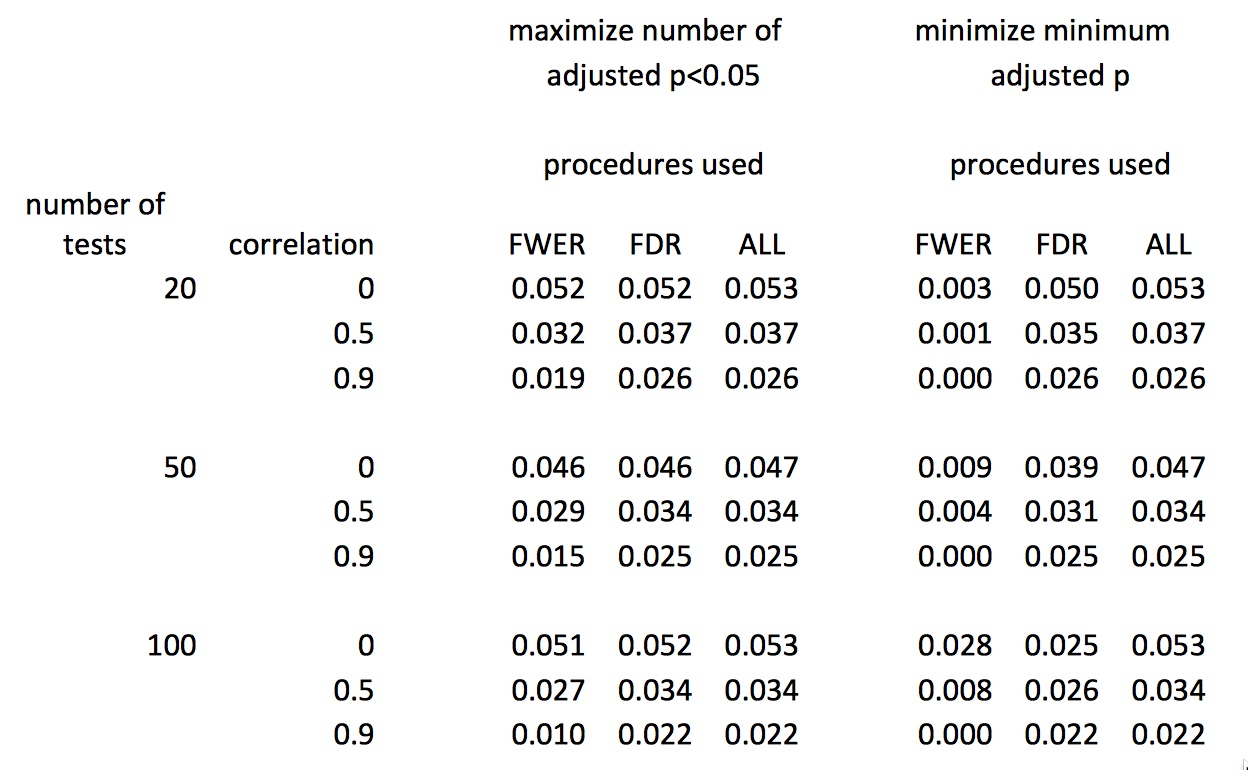
\includegraphics{../figures/rb_table.jpeg}

\end{frame}

\begin{frame}{Perils of post hoc adjustment}
\protect\hypertarget{perils-of-post-hoc-adjustment}{}

Does not distinguish between confirmation and discovery

Are all the primary secondary and subgroup analyses part of the family
of tests examining a treatment effect?

\begin{itemize}
\tightlist
\item
  If so, reduces power for primary outcome
\end{itemize}

\end{frame}

\begin{frame}{Unadjusted \(p\)-values in safety outcomes}
\protect\hypertarget{unadjusted-p-values-in-safety-outcomes}{}

From Metra, et al.~N Engl J Med 2019; 381:716-726 DOI:
10.1056/NEJMoa1801291

\centering

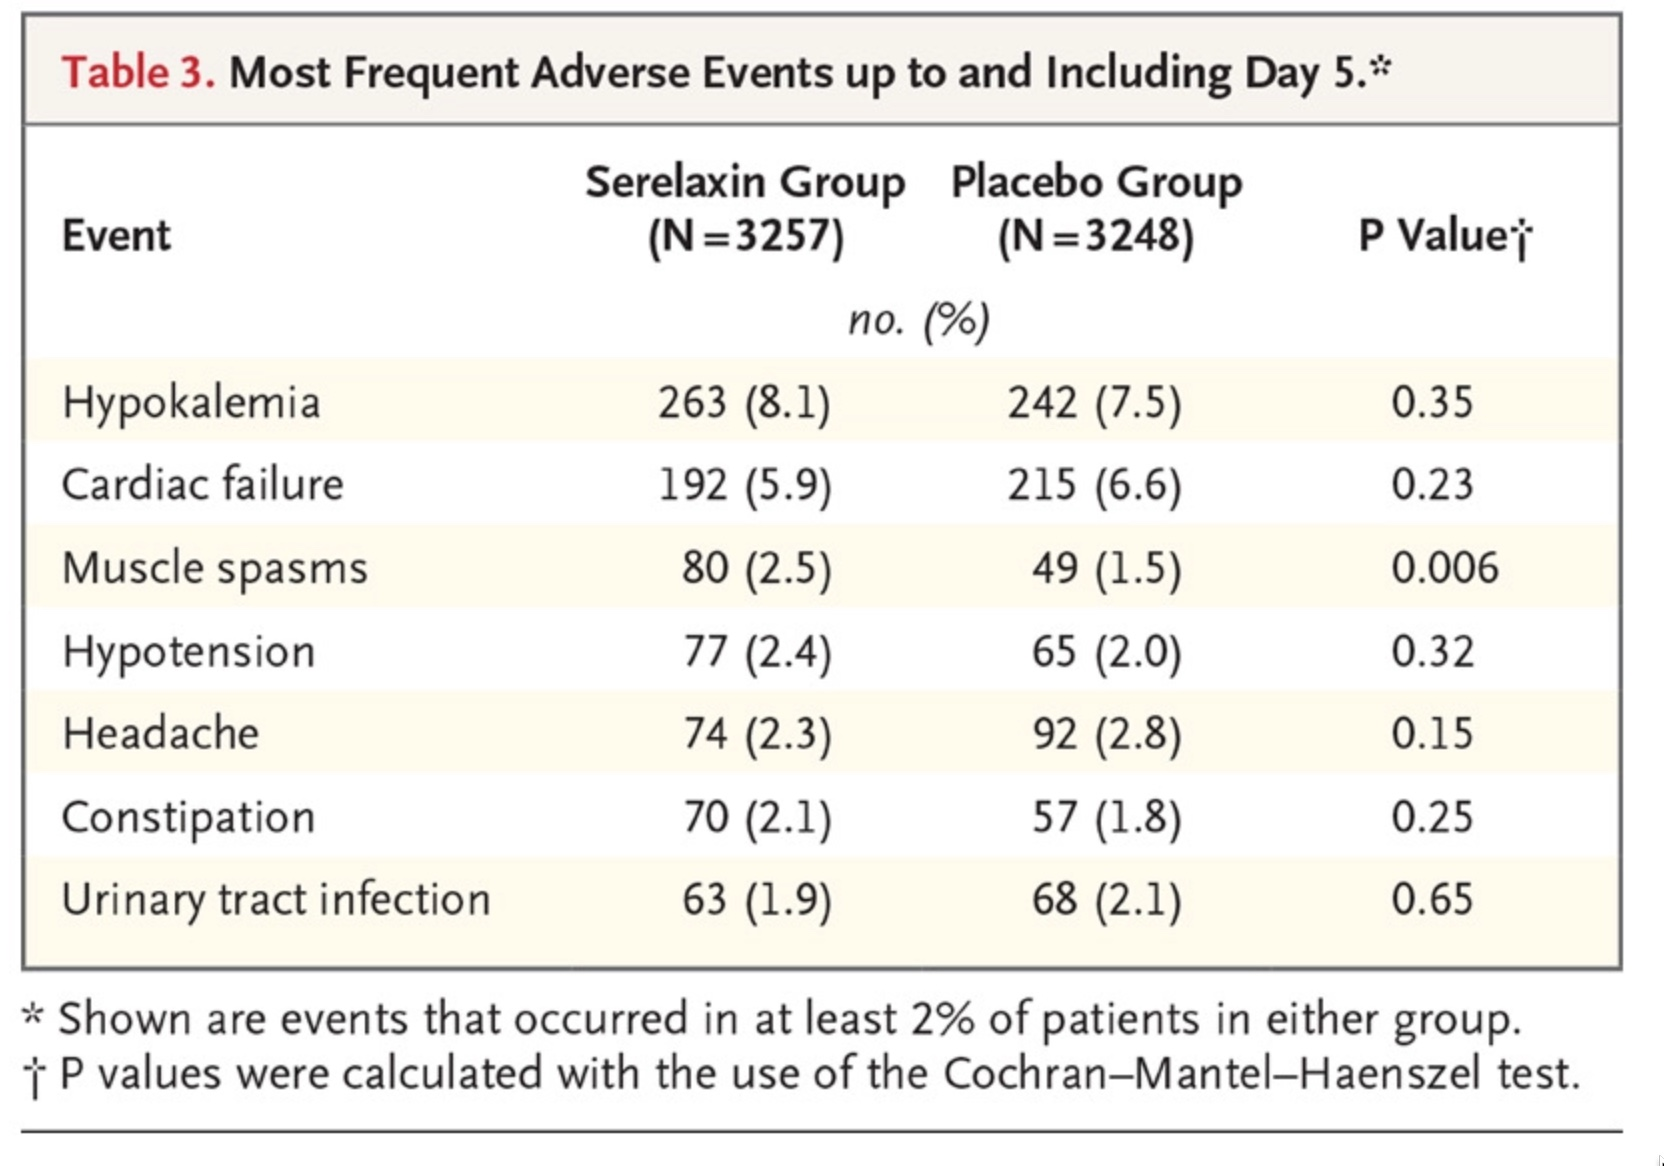
\includegraphics[width=0.7\textwidth,height=\textheight]{../figures/safety_p-values.jpeg}

\end{frame}

\begin{frame}{\(p\) values for interactions}
\protect\hypertarget{p-values-for-interactions}{}

Did we do more harm than good in eliminating \(p\)-values in forest
plots of subgroups?

Deputy editors, authors and some statisticians reluctant to eliminate
these

\begin{itemize}
\item
  Authors and editors found lists of non-significant p-values
  reassuring.
\item
  Easy to recommend that significant p-values be ignored.
\item
  No easy general recommendation for point estimates and confidence
  intervals for inteaction effects.
\end{itemize}

\end{frame}

\begin{frame}{New form of forest plots}
\protect\hypertarget{new-form-of-forest-plots}{}

\centering

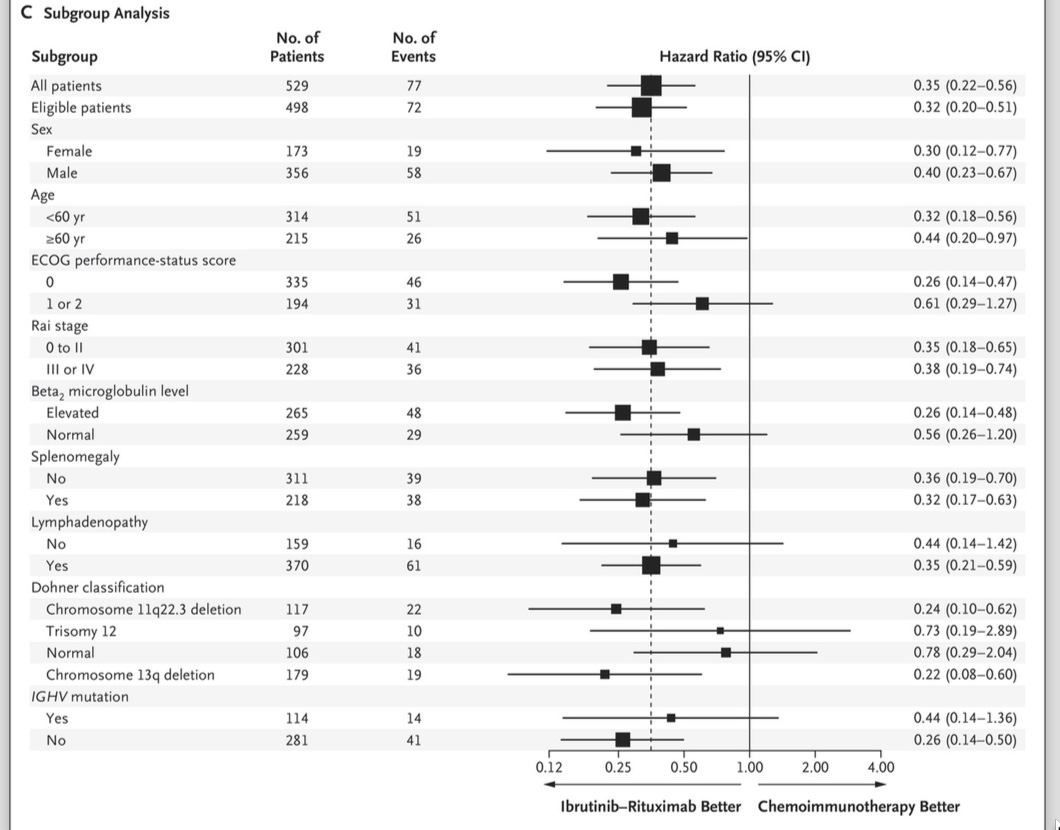
\includegraphics{../figures/shanafelt_subgroups.jpeg}

\end{frame}

\begin{frame}{Before change}
\protect\hypertarget{before-change}{}

\centering

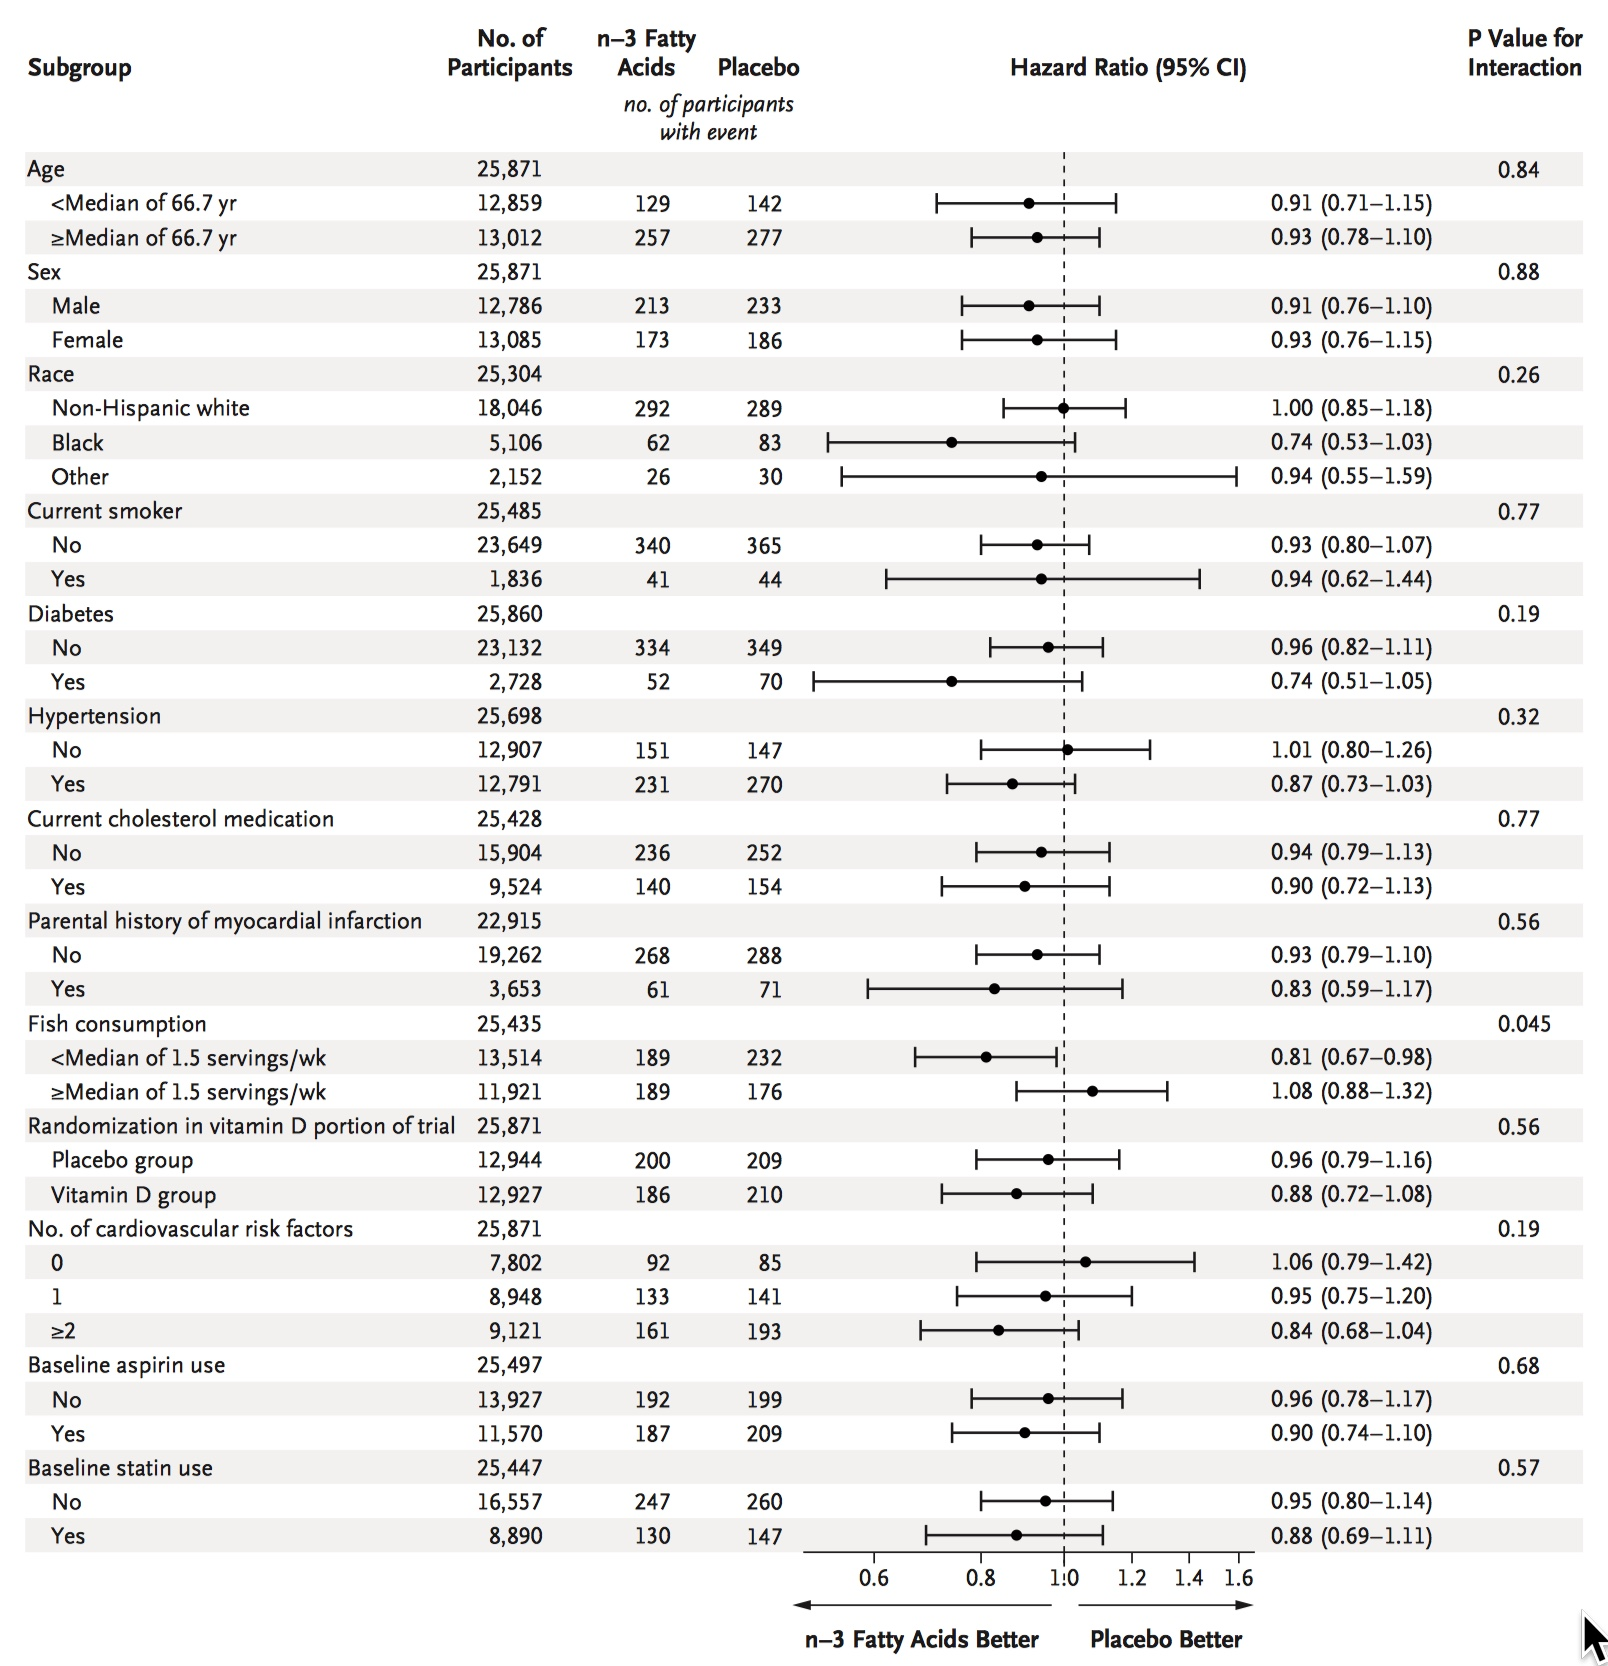
\includegraphics{../figures/vital_subgroups.jpeg}

\end{frame}

\begin{frame}{Perhaps p-values are helpful}
\protect\hypertarget{perhaps-p-values-are-helpful}{}

\centering

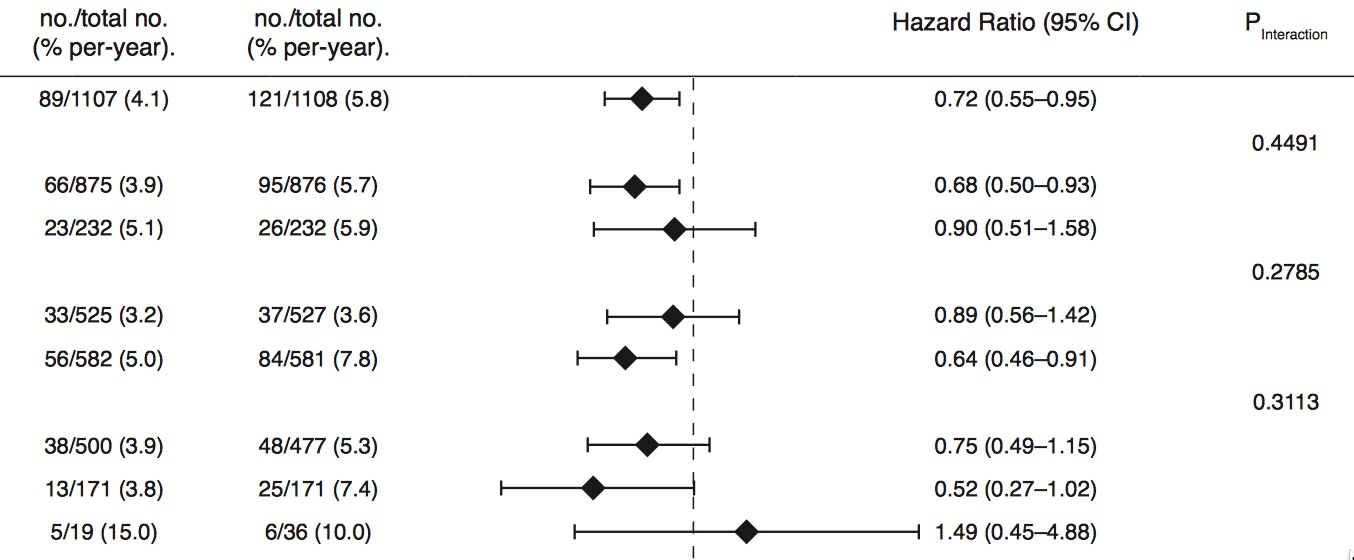
\includegraphics{../figures/me_interaction.jpeg}

\end{frame}

\begin{frame}{Calculating posterior odds (Nat. Human Behavior, Jan
2018)}
\protect\hypertarget{calculating-posterior-odds-nat.-human-behavior-jan-2018}{}

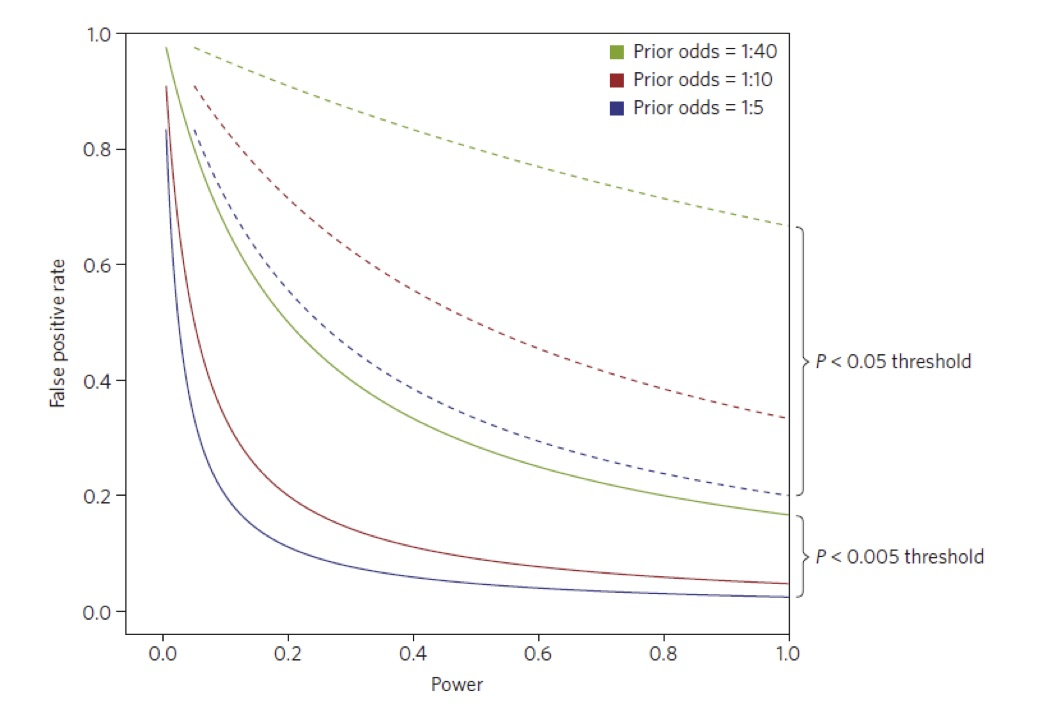
\includegraphics[width=1\textwidth,height=\textheight]{../figures/ppv_threshold.jpeg}

\end{frame}

\begin{frame}{Effect of increasing \(\alpha\)}
\protect\hypertarget{effect-of-increasing-alpha}{}

Prior odds = 1:10, power = 0.80

\begin{longtable}[]{@{}rr@{}}
\toprule
Alpha & False Pos. Prob\tabularnewline
\midrule
\endhead
0.10 & 0.56\tabularnewline
0.15 & 0.65\tabularnewline
0.20 & 0.71\tabularnewline
0.25 & 0.76\tabularnewline
0.40 & 0.83\tabularnewline
0.60 & 0.88\tabularnewline
\bottomrule
\end{longtable}

False Pos. Prob = probability of incorrectly claiming alternative is
true, given data

\end{frame}

\begin{frame}{Assumptions behind the calculations}
\protect\hypertarget{assumptions-behind-the-calculations}{}

Decision to use an intervention based on single trial, single p-value

Prior odds is knowable, at least approximately

There is a simple alternative for which power is relevant

For practicing clinician, is reproducibility the right metric?

\end{frame}

\begin{frame}{Have we made unsupported claims easier?}
\protect\hypertarget{have-we-made-unsupported-claims-easier}{}

Common to encounter phrases in drafts such as

\begin{quote} A consistent pattern for improved survival \ldots was noted across multiple subgroups
\end{quote}

or

\begin{quote}

An exploratory \ldots analysis \ldots of patients who resumed [intervention]  was superior to that of patients who did not

\end{quote}

\end{frame}

\begin{frame}

PDF of slides available at under mskcc\_2019 at

\url{https://github.com/dave-harrington/talks}

\end{frame}

\begin{frame}{Reading}
\protect\hypertarget{reading}{}

\small

Benjamin DJ, et al.~Redefine statistical significance. Nat Hum Behavior
2018;2:6-10. doi: 10.1038/s41562-017-0189-z

Ioannidis JPA. Retiring statistical significance would give bias a free
pass. Nature. 2019;567 (7749):461. \url{doi:10.1038/d41586-019-00969-2}

National Academies of Sciences, Engineering, and Medicine.
Reproducibility and replicability in science. Washington, DC: National
Academies Press, 2019. \url{http://nap.edu/25303}

Wasserstein RL, Schirm AL, Lazar NA. Moving to a world beyond
p\textless{}0.05. Am Stat. 2019;73:1-19.
\url{doi:10.1080/00031305.2019.1583913}

Dmitrienko A, Bretz F, Westfall PH, et al.~Multiple testing methodology.
In: Dmitrienko A, Tamhane AC, Bretz F, eds. Multiple testing problems in
pharmaceutical statistics. New York: Chapman and Hall/CRC Press,
2009:35-98.

\end{frame}

\end{document}
